\documentclass[compressed, presentation, notheorems, 12pt]{beamer}

\newcommand*{\Module}{LatexModules}

% ----------------------------------------------------------
% Preamble
% ----------------------------------------------------------

% Følgende er til koder.
%----------------------------------------------------------
%\begin{lstlisting}[caption=Overskrift på boks, style=Code-C++, label=lst:referenceLabel]
%public void hello(){}
%\end{lstlisting}
%----------------------------------------------------------

%Exstra space
\usepackage{xspace}
%Navn på bokse efterfulgt af \xspace (hvis det skal være mellemrum
%gives det med denne udvidelse. Ellers ingen mellemrum.
\newcommand{\codeTitle}{Code snippet\xspace}

%Pakker der skal bruges til lstlisting
\usepackage{listings}
\usepackage{color}
\usepackage{textcomp}
\definecolor{listinggray}{gray}{0.9}
\definecolor{lbcolor}{rgb}{0.9,0.9,0.9}
\renewcommand{\lstlistingname}{\codeTitle}
\lstdefinestyle{Code}
{
	keywordstyle	= \bfseries\ttfamily\color[rgb]{0,0,1},
	identifierstyle	= \ttfamily,
	commentstyle	= \color[rgb]{0.133,0.545,0.133},
	stringstyle		= \ttfamily\color[rgb]{0.627,0.126,0.941},
	showstringspaces= false,
	basicstyle		= \small,
	numberstyle		= \footnotesize,
%	numbers			= left, % Tal? Udkommenter hvis ikke
	stepnumber		= 2,
	numbersep		= 6pt,
	tabsize			= 2,
	breaklines		= true,
	prebreak 		= \raisebox{0ex}[0ex][0ex]{\ensuremath{\hookleftarrow}},
	breakatwhitespace= false,
%	aboveskip		= {1.5\baselineskip},
  	columns			= fixed,
  	upquote			= true,
  	extendedchars	= true,
 	backgroundcolor = \color{lbcolor},
	lineskip		= 1pt,
%	xleftmargin		= 17pt,
%	framexleftmargin= 17pt,
	framexrightmargin	= 0pt, %6pt
%	framexbottommargin	= 4pt,
}

%Bredde der bruges til indryk
\usepackage{calc}


% Forskellige styles for forskellige kodetyper
\usepackage{caption}
\DeclareCaptionFont{white}{\color{white}}
\DeclareCaptionFormat{listing}%
{\colorbox[cmyk]{0.43, 0.35, 0.35,0.35}{\parbox{\textwidth - 6pt}{\hspace{5pt}#1#2#3}}}

\captionsetup[lstlisting]
{
	format			= listing,
	labelfont		= white,
	textfont		= white, 
	singlelinecheck	= false, 
	width			= \textwidth - \marginparsep,
	margin			= 0pt, 
	font			= {bf,footnotesize}
}

\lstdefinestyle{Code-C} {language=C, style=Code}
\lstdefinestyle{Code-Java} {language=Java, style=Code}
\lstdefinestyle{Code-C++} {language=[Visual]C++, style=Code}
\lstdefinestyle{Code-VHDL} {language=VHDL, style=Code}
\lstdefinestyle{Code-Bash} {language=Bash, style=Code}
\lstdefinestyle{Code-Matlab} {language=Matlab, style=Code}
\lstdefinestyle{Code-Prolog} {language=Prolog, style=Code}
%Speciel skrift for enkelt linje kode
%--------------------------------------------------
%Udskriver med fonten 'Courier'
%Mere info her: http://tex.stackexchange.com/questions/25249/how-do-i-use-a-particular-font-for-a-small-section-of-text-in-my-document
%Eksempel: Funktionen \code{void Hello()} giver et output
%--------------------------------------------------
\newcommand{\code}[1]{{\fontfamily{pcr}\selectfont #1}}

%Standard path to search for pictures
%--------------------------------------------------
%\begin{figure}[hbtp]
%\centering
%\includegraphics[width =0.9 \textwidth]{filnavn-for-png}
%\caption{Titel}
%\label{fig:referenceNavn}
%\end{figure}
%--------------------------------------------------

\usepackage{graphicx}
\usepackage{subcaption}
\usepackage{float}

%Paths the pictures can be located
\graphicspath{
	{../Figures/}
	{Figures/}
}
% 
%FixMe pakken viser små kommentarer, hvor der skal rettes
%--------------------------------------------------
%Brug med følgende: \fxnote{det her skal uddybes!}
%Se liste over alle fixMe's: \listoffixmes
%Erstat 'draft' med 'final' for at fjerne alle kommentarer
%--------------------------------------------------
\usepackage[footnote,draft,danish,silent,nomargin]{fixme}

% \input{\Module/FrontPageSetup}
%%Makes linebreak after a \paragraph{} automatically and possible
%
%http://www.latex-community.org/forum/viewtopic.php?f=5&t=1383

\makeatletter
\renewcommand\paragraph{\@startsection{paragraph}{4}{\z@}%
  {-3.25ex\@plus -1ex \@minus -.2ex}%
  {1.5ex \@plus .2ex}%
  {\normalfont\normalsize\bfseries}}
\makeatother
% %Seperated files
%--------------------------------------------------
%Opret filer således:
%\documentclass[Navn-på-hovedfil]{subfiles}
%\begin{document}
% Indmad
%\end{document}
%
% I hovedfil inkluderes således:
% \subfile{navn-på-subfil}
%--------------------------------------------------
\usepackage{subfiles}
% 
%Dybde på indholdsfortegnelse
%----------------------------------------------------------
%Chapter, section, subsection, subsubsection
%----------------------------------------------------------
\setcounter{secnumdepth}{3}
\setcounter{tocdepth}{3}
% %Tables
%----------------------------------------------------------
\usepackage{tabularx}
\usepackage{array}
\usepackage{multirow} 
\usepackage{multicol} 
\usepackage{booktabs}
\usepackage{wrapfig}
\usepackage{longtable}
%\renewcommand{\arraystretch}{1.5}

%Colors in tables
\usepackage{color, colortbl}
\definecolor{gr}{gray}{0.9}
%\rowcolor{gr}
% 

%--------------------------------------------------
%\begin{TestCaseIntro}
%\TCprep{Preperation of sorts \\Anything here}
%\TCdesc{Description of what is ablut to happen}
%\end{TestCaseIntro}
%--------------------------------------------------
\newcommand{\TCdescWidth}{0.15 \textwidth}
\newcommand{\TCIntroWidth}{0.8\textwidth}
\newcommand{\TCprep}[1]{\textbf{Forberedelse:} & \parbox[t]{\TCIntroWidth}{#1}}
\newcommand{\TCdesc}[1]{\\ \textbf{Beskrivelse:} & \parbox[t]{\TCIntroWidth}{#1}}

\newenvironment{TestCaseIntro}
{\begin{longtable}{p{\TCdescWidth} p{\TCIntroWidth}}}
{\end{longtable}}
%--------------------------------------------------



%--------------------------------------------------
%\begin{TestCase}
%\TC
%{Steps}
%{Aktion to take}
%{Expectation}
%{Leave blank}
%\end{TestCase}
%--------------------------------------------------
\newcommand{\TCsteps}{0.05 \textwidth}
\newcommand{\TCexpected}{0.38 \textwidth}
\newcommand{\TCmethod}{0.38 \textwidth}
\newcommand{\TCsucces}{0.08 \textwidth}

\newenvironment{TestCase}
{\begin{longtable}{ p{\TCsteps}  p{\TCexpected} p{\TCmethod} p{\TCsucces} }
\hline \textbf{Trin} & \textbf{Metode} & \textbf{Forventet} & \textbf{Succes}}
{\\ \hline \end{longtable}}

\newcommand{\TC}[4]{\\ \hline \parbox[t]{\TCsteps}{#1} & \parbox[t]{\TCmethod}{#2} &\parbox[t]{\TCexpected}{#3}&  \parbox[t]{\TCsucces}{#4} }
%--------------------------------------------------
%Text typesetting
%--------------------------------------------------------
\usepackage[T1]{fontenc} 	% Can use danish characters
\usepackage[utf8]{inputenc} % Input encoding. Can be used on Linux, Mac and Windows         
\usepackage[danish]{babel} 	% Split words accoding to English
\usepackage{lmodern} 		% Font

\usepackage[activate={true,nocompatibility},final,tracking=true,kerning=true,spacing=true,factor=1100,stretch=10,shrink=10]{microtype}


% Enumeration
%-------------------------------------------------------------------
% Use both packages
\usepackage{enumerate}
\usepackage[shortlabels]{enumitem}
%-------------------------------------------------------------------

% Indent on empty line break (more than 1)
%-------------------------------------------------------------------
\setlength\parindent{0pt} 	% No indent
\setlength\parskip{12pt} 	% More than a single line break will give ONE linebreak.
%-------------------------------------------------------------------

% Microtype package
%-------------------------------------------------------------------
% See http://www.khirevich.com/latex/microtype/ for explanation

\SetExtraKerning[unit=space]
    {encoding={*}, family={bch}, series={*}, size={footnotesize,small,normalsize}}
    {\textendash={400,400}, 		% en-dash, add more space around it
     "28={ ,150}, 					% left bracket, add space from right
     "29={150, }, 					% right bracket, add space from left
     \textquotedblleft={ ,150}, 	% left quotation mark, space from right
     \textquotedblright={150, }} 	% right quotation mark, space from left

\SetTracking{encoding={*}, shape=sc}{40}

\let\newTOC\tableofcontents
\renewcommand{\tableofcontents}
{
	\microtypesetup{protrusion=false} 	% disables protrusion locally in the document
	\newTOC			 					% prints Table of Contents
	\microtypesetup{protrusion=true} 	% enables protrusion
}
%-------------------------------------------------------------------




%%URL kommandoer og sidetal farve
%%Kaldes med \url{www...}
%\usepackage{color} %Skal også bruges
\usepackage{hyperref}
\hypersetup{ 
	colorlinks	= true, 	% false: boxed links; true: colored links
    urlcolor	= blue,		% color of external links
    linkcolor	= black, 	% color of page numbers
    citecolor	= blue,
}


%\usepackage[left=2cm,right=2cm,top=2.5cm,bottom=2cm]{geometry}

\linespread{1.5}

\newcommand{\HRule}{\rule{\linewidth}{0.8mm}}

%Tekst i fotter
\usepackage{lastpage} %Finds last page number
\usepackage{xspace} %Inserts necesary space bestween the page number, the dash and the total pagenumber
\newcommand{\footerText}{\thepage\xspace /\pageref{LastPage}}
%%Setup for the 'memoir' package (replace 'article')

%Margin
\usepackage[left=3cm,right=2cm,top=2.5cm,bottom=2cm]{geometry}

\linespread{1.5}

\newcommand{\HRule}{\rule{\linewidth}{0.8mm}}

%Tekst i fotter
\usepackage{lastpage} %Finds last page number
\usepackage{xspace} %Inserts necesary space bestween the page number, the dash and the total pagenumber
\newcommand{\footerText}{\thepage\xspace /\pageref{LastPage}}


% Specific chapter style.
% See more at: ftp://ftp.tex.ac.uk/tex-archive/info/MemoirChapStyles/MemoirChapStyles.pdf
\chapterstyle{hangnum}

\nouppercaseheads
\makepagestyle{mystyle} 

\makeevenhead{mystyle}{}{\\ \leftmark}{} 
\makeoddhead{mystyle}{}{\\ \leftmark}{} 
\makeevenfoot{mystyle}{}{\footerText}{} 
\makeoddfoot{mystyle}{}{\footerText}{} 
\makeatletter
\makepsmarks{mystyle}{% Overskriften på sidehovedet
  \createmark{chapter}{left}{shownumber}{\@chapapp\ }{.\ }} 
\makeatother
\makefootrule{mystyle}{\textwidth}{\normalrulethickness}{0.4pt}
\makeheadrule{mystyle}{\textwidth}{\normalrulethickness}

\makepagestyle{plain}
\makeevenhead{plain}{}{}{}
\makeoddhead{plain}{}{}{}
\makeevenfoot{plain}{}{\footerText}{}
\makeoddfoot{plain}{}{\footerText}{}
\makefootrule{plain}{\textwidth}{\normalrulethickness}{0.4pt}

\pagestyle{mystyle}

%%----------------------------------------------------------------------
%
%%Redefining chapter style
%%\renewcommand\chapterheadstart{\vspace*{\beforechapskip}}
%\renewcommand\chapterheadstart{\vspace*{10pt}}
%\renewcommand\printchaptername{\chapnamefont }%\@chapapp}
%\renewcommand\chapternamenum{\space}
%\renewcommand\printchapternum{\chapnumfont \thechapter}
%\renewcommand\afterchapternum{\space: }%\par\nobreak\vskip \midchapskip}
%\renewcommand\printchapternonum{}
%\renewcommand\printchaptertitle[1]{\chaptitlefont #1}
\setlength{\beforechapskip}{0pt} 
\setlength{\afterchapskip}{0pt} 
%\setlength{\voffset}{0pt} 
\setlength{\headsep}{25pt}
%\setlength{\topmargin}{35pt}
%%\setlength{\headheight}{102pt}
%\setlength{\textheight}{302pt}
\renewcommand\afterchaptertitle{\par\nobreak\vskip \afterchapskip}
%%----------------------------------------------------------------------



\title{Group 3's PTP system}
\subtitle{Slides and presentation}
\author[Author, Anders] % (optional, for multiple authors)
{L.~Brøsted \and R.~Bækgaard \and M.~Manø \and C.~Werge}
\institute
{
  Aarhus University \\
  School of Engineering
}
\date{TIMICO, 2014}
\subject{DDS}

\begin{document}
 	\frame{\titlepage}

\begin{frame}
\frametitle{Table of Contents}
\tableofcontents%[currentsection]
\end{frame}

\section{Theory of DDS}

\begin{frame}{Results}

\begin{figure}[hbtp]
\centering
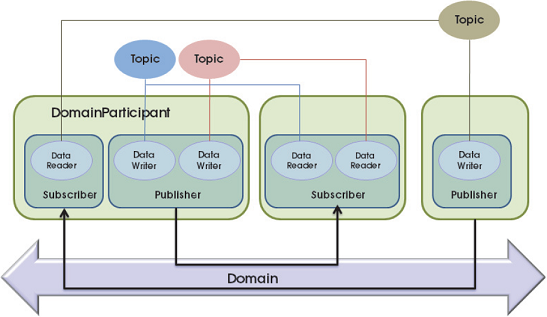
\includegraphics[width =0.9 \textwidth]{RTI_EntityOverview_small}
\caption{DCPS model}
\end{figure}


\end{frame}


\begin{frame}{Mapping PTP to DDS 1/3}
\begin{itemize}
	\item 3 topics
	\begin{itemize}
		\item "PTP" - Broadcast master(s) to slave(s), explicit
		\begin{itemize}
			\item SYNC, FOLLOWUP
		\end{itemize}
		\item "PTPRequest" - slave to master, implicit
		\begin{itemize}
			\item DELAYREQUEST
		\end{itemize}
		\item "PTPReply" - master to slave, implicit
		\begin{itemize}
		 	\item DELAYRESPONSE
		 \end{itemize} 
	\end{itemize}

	\item  1 domain - id 0
\end{itemize}
\end{frame}



\begin{frame}{Mapping PTP to DDS 2/3}
\begin{itemize}
	\item Master
	\begin{itemize}
		\item DomainParticipant
		\item  Publisher
		\item Topic("PTP")
		\item MsgDataWriter
		\item Replier (abstracts Subscriber + Publisher and DataReader + DataWriter)
		\begin{itemize}
			\item  Topics "PTPRequest" + "PTPReply"
		\end{itemize}
	\end{itemize}
\end{itemize}
\end{frame}



\begin{frame}{Mapping PTP to DDS 3/3}
\begin{itemize}
	\item Slave
	\begin{itemize}
		\item DomainParticipant
		\item  Subscriber
		\item Topic("PTP")
		\item MsgDataReader
		\item Requester (abstracts Subscriber + Publisher and DataReader + DataWriter)
		\begin{itemize}
			\item  Topics "PTPRequest" + "PTPReply"
		\end{itemize}
	\end{itemize}
\end{itemize}
\end{frame}
	
\section{The slave}
	\begin{frame}{The slave's role}	

	\begin{itemize}
		\item Receive timestamps from the master
		\item Make delay request
		\item Keep track of time
	\end{itemize}
	
	\end{frame}


\subsection{IDL generation}
	\begin{frame}[containsverbatim]{The IDL file generated  with RTIDDSGEN}

	\begin{lstlisting}[style=Code-C++]
module PTP
{
  enum MsgType
  {
    SYNC,
    FOLLOWUP,
    DELAYREQUEST,
    DELAYRESPONSE
  };
  struct Msg
  {
    MsgType type;         
    unsigned long long value;     
  };
};
	\end{lstlisting}
	\end{frame}



\subsection{Slave functions}

	\begin{frame}[containsverbatim]{Slave main loop}
	
	\begin{lstlisting}[style=Code-C++]
using(var slave = new Slave())
{
	slave.setup(domain_id: 0);
	
	const int receive_period = 2000; 
	while (keepRunning)
	{
		long delayTs, delayTm;
		slave.SendRequest(out delayTs, out delayTm);
		slave.setDelay(delayTs, delayTm);

		Thread.Sleep(receive_period);
	}
}
	\end{lstlisting}

	\end{frame}




	\begin{frame}[containsverbatim]{Handle the data received}
	\begin{lstlisting}[style=Code-C++]
void handleDataReceived(Msg data)
{
   switch (data.type)
	{
		case SYNC:
			syncTs = clock.Now.Ticks;
			break;
		case FOLLOWUP:
			clock.Offset = syncTs - data.value - Delay;
			syncTm = data.value;
			break;
	}
}
	\end{lstlisting}
	\end{frame}





	\begin{frame}[containsverbatim]{Sendrequest 1/2}
	\begin{lstlisting}[style=Code-C++]
void SendRequest(out long ts, out long tm)
{
	var request = new Msg { type = DELAYREQUEST };
	ts = clock.Now.Ticks;
	requester.SendRequest(request);

	var reply = requester.CreateReplySample();
	var received = requester.ReceiveReply(reply, maxWait);

	\end{lstlisting}
	\end{frame}



	\begin{frame}[containsverbatim]{Sendrequest 2/2}
	\begin{lstlisting}[style=Code-C++]
	if (received)
	{
		if (reply.Info.valid_data)
		{
			if(reply.Data.type == DELAYRESPONSE)
			{
				tm = reply.Data.value;
			}
		}
	}
}
	\end{lstlisting}
	\end{frame}

\begin{frame}[containsverbatim]{Simulating slave clock}
	\begin{lstlisting}[style=Code-C++]
long GetTime()
{
	var elapsed = sw.Elapsed.Ticks;
	now += elapsed - lastElapsed;

	lastElapsed = elapsed;

	return now;
}
	\end{lstlisting}
	\end{frame}

\section{Master}

	\begin{frame}{The master}
	\begin{itemize}
		\item Must send its time to the slave.
		\item Must answer the slave when asking for time.
	\end{itemize}
	\end{frame}


\subsection{Master functions}
	\begin{frame}[containsverbatim]{Main}
	\begin{lstlisting}[style=Code-C++]
using (var master = new Master())
{
	master.setup(domain_id: 0);
	const int send_period = 485; 

	while (keepRunning)
	{
		var tm = getCurrentTime();

		master.sendSync(tm + jitter());
		master.sendFollowup(tm);						

		Thread.Sleep(send_period);
	}
}
	\end{lstlisting}
	\end{frame}

 	

	\begin{frame}[containsverbatim]{Broadcasting SYNC to the slaves}
	\begin{lstlisting}[style=Code-C++]
public void sendSync(long estimatedTm)
{
	instance.type = MsgType.SYNC;
	instance.value = estimatedTm;
	writer.write(instance, ref instance_handle);
}
	\end{lstlisting}

	The function \code{sendFollowup(long tm)} is very similar.
	\end{frame}

\begin{frame}[containsverbatim]{Response from slave}
	\begin{lstlisting}[style=Code-C++]
class MsgReplierListener : SimpleReplierListener<Msg, Msg>
{
	Msg reply = new Msg {type=DELAYRESPONSE};

	Msg OnRequestAvailable(Sample<Msg> req)
	{
		reply.type = DELAYRESPONSE;
		reply.value = Master.getCurrentTime();
		return reply;
	}
}
	\end{lstlisting}

	\end{frame}


\section{Results}
\begin{frame}{Results}

\begin{figure}[hbtp]
\centering
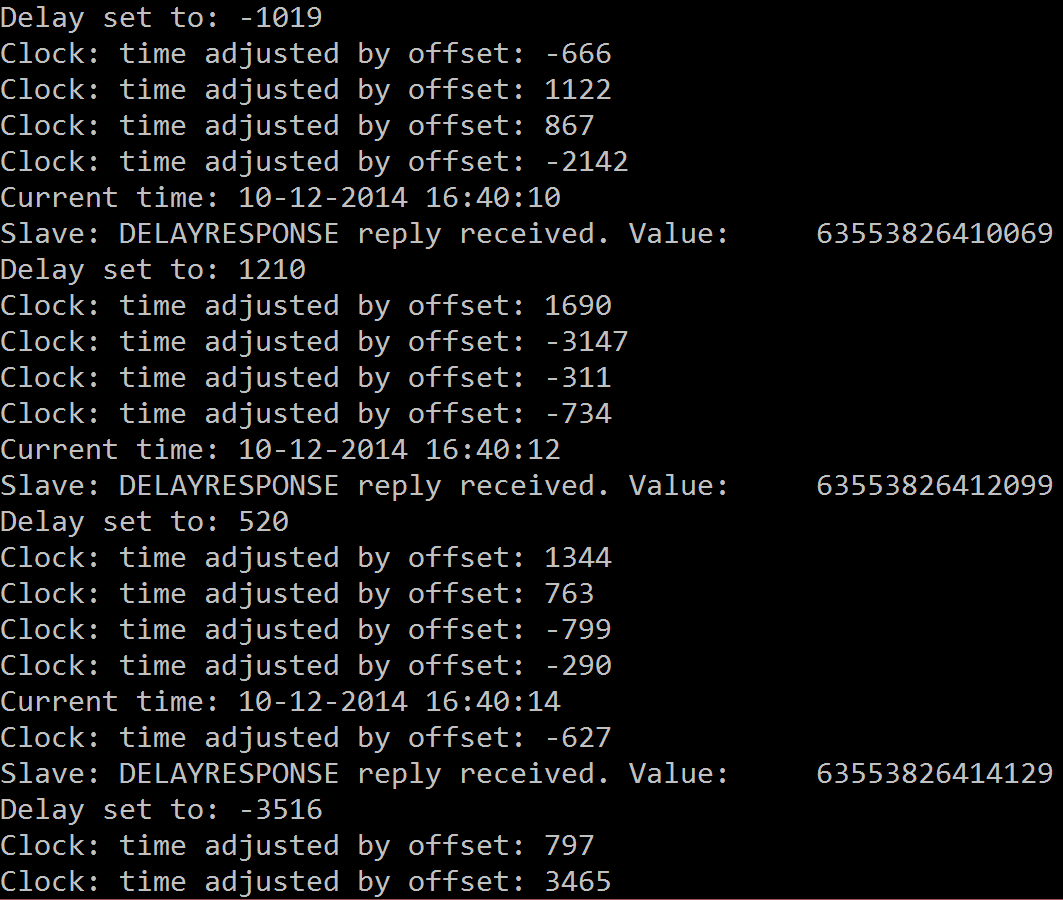
\includegraphics[width = 0.82 \textwidth]{SlaveScreen}
\caption{Results}
\end{figure}


\end{frame}



\end{document}
